
\glsresetall

\chapter{Introduction}
\label{ch:intro}

The realm of nuclear security involves parallel efforts in nonproliferation
(verification of treaty compliance, monitoring for smuggling, proper storage and
transportation of nuclear materials), cyber security, minimizing stocks of
weaponizable materials, disaster response training, and nuclear forensics. All
of these efforts have been continually improving, but there was a gap regarding
the ability of the \gls{US} to coordinate and respond to a nuclear incident,
especially with the technical portion of nuclear forensics: characterization and
analysis. After all, the first textbook on the topic was published in 2005
\cite{nftext_2005}. In 2006, the \gls{US} \gls{DHS} founded the \gls{NTNFC}
within the \gls{DNDO}, with the mission to establish a robust nuclear forensics
capability by attributing radioactive materials with demonstrable proof. This
endeavor was and is highly dependent on inter-agency cooperation. In 2017 \--
2018, the \gls{DNDO} was absorbed into the newer \gls{CWMD} office, and in 2019,
much of the nuclear forensics research operation was moved to multiple offices
within the \gls{DOE} \gls{NNSA}. 

Multiple fields contribute to a nuclear forensics capability, such as
radiochemical separations, material collection techniques, detector technology,
material library development, and identifying forensic signatures. These needs
vary based on whether the material being collected is post-detonation (e.g.,
bomb debris) or pre-detonation (e.g., \gls{SNF}).  In the
pre-detonation realm, this project focuses on statistical methods to to model
the production history of a nuclear material using measurements of nuclides
present in the \gls{SNF}.

\gls{SNF} is identified in this work by focusing on four characteristics in
particular that can potentially provide material attribution: reactor type,
burnup, initial \gls{U235} enrichment, and time since fuel irradiation. 
\begin{enumerate}
  \item The \textbf{reactor type} is classified as one of the three most common
        types of commercial power reactors: \gls{PWR}, \gls{BWR}, or \gls{PHWR}.
  \item The \textbf{burnup} describes how much energy was produced by the fuel,
        taking on the units \textit{megawatt-days (or gigawatt-days) per metric 
        ton of heavy metal (or initial uranium)}; it is referred to in this work 
        as $MWd/MTU$, and sometimes $GWd/MTU$.  
  \item The \textbf{enrichment} is the percentage of \gls{U235} with respect to
        the entire amount of uranium in the fuel, and is reported as $\%U235$. 
  \item Lastly, the \textbf{time since irradiation} is defined as how long the
        fuel has been out of the reactor core, and is discussed usually in $days$,
        but sometimes $years$. It may also be referred to as cooling time. 
\end{enumerate}

\section{Motivation}
\label{sec:motivation}

Preventing nuclear terrorism is important work that has a role along the entire
lifetime of nuclear material, from the beginning (e.g., enrichment facility
inspections) to the end (e.g., \gls{SNF} management). The \gls{IAEA} tracks
reports of radioactive material out of regulatory control via the \gls{ITDB}
\cite{itdb}, and the incidents that are confirmed or likely to be related to
trafficking or malicious use are summarized in Figure \ref{fig:incidents}.
These are the circumstances in which a robust nuclear forensics capability is
beneficial.

\begin{figure}[!tbh]
  \makebox[\textwidth][c]{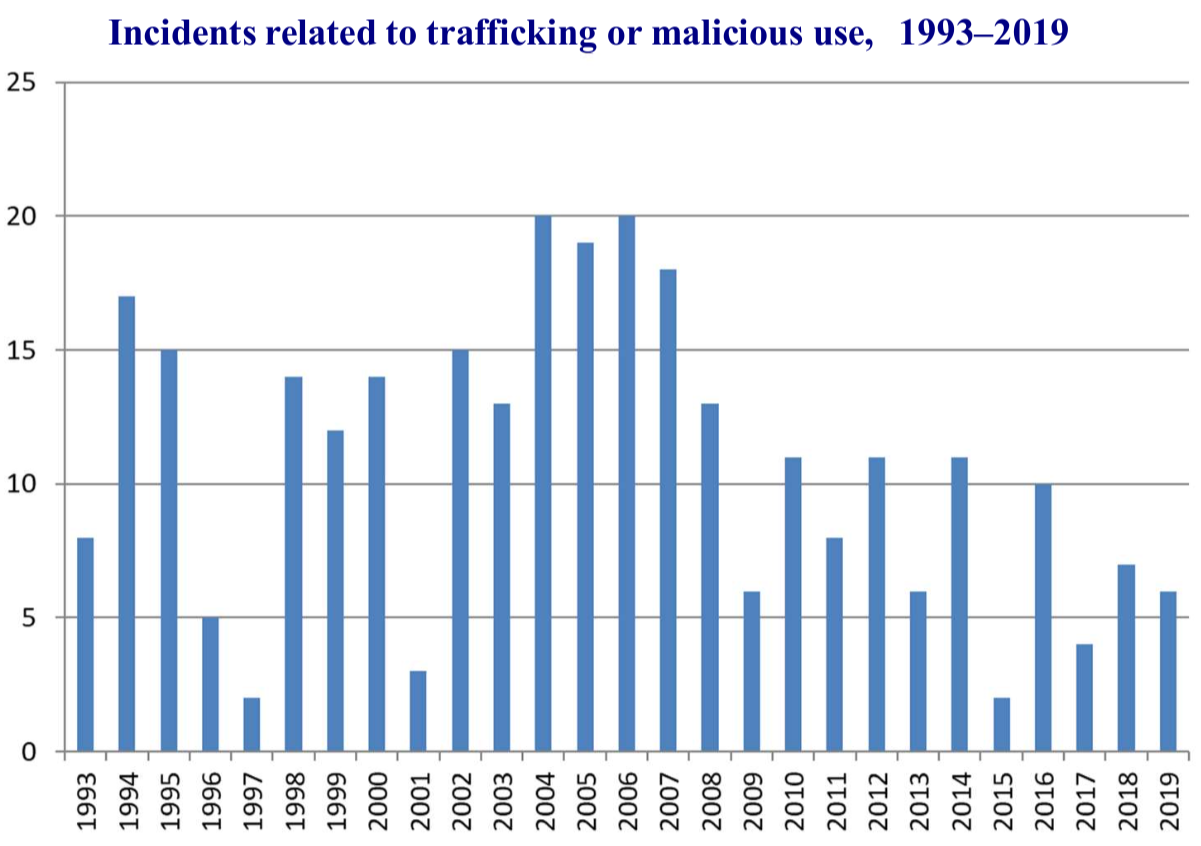
\includegraphics[width=\linewidth]{./chapters/intro/nucleartrafficking.png}}
  \caption{Incidents reported to the \acrshort{IAEA} \acrshort{ITDB} related to 
           malicious use. Included are highly enriched uranium (12), 
           plutonium (2), plutonium-beryllium neutron sources (5) 
           \cite{itdb}}
  \label{fig:incidents}
\end{figure}

Nuclear forensics is an important aspect of deterring nuclear terrorism even
though it is not, at first glance, obvious preventative nuclear security.  The
most common defense of the field is that nuclear forensics deters state actors,
not terrorist organizations. While it is true that a strong capability
encourages governments to be more active in prevention of nuclear terrorism, it
can also deter the terrorist organizations as well by increasing their chances
of failure. Small destructive successes tend to be more valued than high-risk
mass destruction. Nuclear forensics can also assist in cutting off certain
suppliers of nuclear materials or technologies (e.g., nuclear specialists that
are only involved for financial reasons, access to state suppliers), building a
concrete barrier to nuclear terrorism.  Therefore, nuclear forensics is
considered to impede nuclear terrorism in both tangible and abstract ways
\cite{aps_aaas_forensics}.

Following the prevention value of nuclear forensics, it is important to
understand the process of the technical portion of the investigation and how
that can be improved.  In the event of a nuclear incident, such as the
retrieval of stolen \gls{SNM} or the detonation of a dirty bomb,
it is necessary to learn as much as possible about the source of the materials
in a timely manner. In the case of non-detonated \gls{SNM}, knowing the
processes that produced it is crucial to determine the chain of custody of the
interdicted material.  Section \ref{sec:nfneeds} covers the specific needs of
the nuclear forensics community for \gls{SNF} provenance, and Section
\ref{sec:statscontrib} discusses how computational approaches are useful, with
a focus on why statistical methods in particular are being pursued. 

\subsection{Needs in Nuclear Forensics}

\begin{frame}
  \frametitle{Nuclear Forensics Investigations}
  \begin{minipage}[t]{0.5\textwidth}
    \textbf{Post-detonation}
    \begin{itemize}
      \item Collection: debris, swipe samples
      \item Characterization: rapid analysis of isotope ratios
      \item Goals
      \begin{itemize}
        \item Inverse problem: reconstruct weapon design/yield
        \item Safety: informing disaster response
      \end{itemize}
      \item Data evaluation
    \end{itemize}
  \end{minipage}%
  \pause
  \begin{minipage}[t]{0.5\textwidth}
    \textbf{Pre-detonation}
    \begin{itemize}
      \item Collection: depends on intercepted material
      \item \boxalert{Characterization:} non-destructive and destructive
      \item Goals:
      \begin{itemize}
        \item \boxalert{Inverse problem:} material chain of custody
        \item Safety: material handling and security
      \end{itemize}
      \item \boxalert{Data evaluation}
    \end{itemize}
  \end{minipage}
\end{frame}


\begin{frame}
  \frametitle{Nuclear Forensics as an Inverse Problem}
  Necessary to determine the quality of prediction

  Use Bayes' Framework:
  $$ P(A|B) = \frac{P(B|A)P(A)}{P(B)} $$
  $$ P(M|D) = \frac{P(D|M)P(M)}{P(D)} $$
\end{frame}


\label{sec:nfneeds}

\subsection{Contribution of Statistical Methods}
As previously mentioned, there are two main issues that are being addressed for
forensics of \gls{SNF}: database issues and speed of characterization. Many
have begun considering computational approaches to nuclear forensics problems,
such as the INDEPTH tool for inverse depletion and decay analysis
\cite{weber_2006, weber_2010, weber_2011}. This tool uses an iterative
optimization method involving many forward simulations to obtain reactor
parameters of interest given some initial values. 

Another approach utilizes artificial intelligence to solve nuclear forensics
problems, such as implementing searching algorithms for the database comparison
step \cite{gey_search} and machine learning for determining reactor parameters
from \gls{SNF} characteristics \cite{dayman_feasibility_2013, nicolaou_2006,
nicolaou_2009, nicolaou_2014, robel_2009, jones_viz_2014, jones_snf_2014}.  A
variety of statistical and machine learning tools have been used to
characterize spent fuel by predicting categories or labels (reactor type, fuel
type) as well as predicting values (burnup, initial enrichment, or cooling
time) The former uses classification algorithms and the latter uses regression
algorithms. Many algorithms can be applied to both cases.

A typical (supervised) machine learning workflow would take a set of training
data with labels or values inserted into some statistical learner, calculate
some objective, minimize or maximize that objective, and provide some model
based on that output. Then a test set (with known values) is provided to the
model so that its performance can be evaluated and finalized. After model
finalization, a user can provide a single instance and a value can be predicted
from that. \todo{insert ML schematic}

To obtain reliable models, one must 1. choose/create a training set carefully
and 2. study the impact of various algorithm parameters on the error. Many
algorithms are developed on an assumption that the training set will be
independent and identially distributed (i.i.d.). [Aside: there are ways to
handle skewed data sets] This is important so that the model does not overvalue
or overfit a certain area in the training space. Additionally, algorithm
performance (or error) can be optimized with respect to training set size,
number of features, or algorithm parameters (regularization terms, etc).  These
are known as diagnostic plots. When plotting the training and testing error
with respect to the number of instances, this is known as a learning curve.
When plotting these errors with respect to the number or features or algorithm
parameters, this is known as a validation curve. \todo{insert example
diagnostic plot?}

Algorithm choice is usually based on what is being predicted and intuition
regarding strengths and weaknesses.  For the sake of comparison (i.e. weak
validation), some machine learning approaches here are based on previous work
\cite{dayman_feasibility_2013} while also extending to a more complex model
via an algorithm that is known to handle highly dimensional data sets well.
Thus, this paper investigates three regression algorithms: nearest neighbor,
ridge, and support vectors.


It is first important to determine if statistical methods can
overcome the inherent database deficiencies. Next, the statistical methods must
be considered in such a way as to represent a real-world scenario. Although
mass spectrometry techniques provide extremely accurate isotopic information
for analytical methods, they are time-consuming and more expensive. And
although gamma spectroscopy can give extremely fast results cheaply, it only
measures certain radiological signals and is influenced by many environmental
factors, storage, and self-attenuation. As different machine learning
algorithms and parameters are investigated, this work focuses on probing the
amount of information required to obtain realistic results.

Because creating databases from real measurements to represent reactor
technologies from around the world is impossible, the database in this study
will be created from high-fidelity simulations via ORIGEN irradiation and
depletion \todo{check actual name of code part used}. In the simulation and
statistical learning paradigm, we need to determine how much information to
what quality is needed to train a machine-learned model; the model must give
appropriate predictions of reactor parameters given a set of measurements from
a test sample of interdicted \gls{SNF}. Of interest to an entity trying to
create a weapon is partially irradiated fuel if they have plutonium separations
capabilities or any radioactive substance in the case of a dirty bomb.
Addressing the former, a set of simulations of \gls{SNF} at different burnups
and cooling times will comprise the database.\todo{rewrite to be clearer}

Can the algorithm overcome the deficiencies of gamma detection and still
provide useful results? Or does it need more information, e.g., exact
isotopics? First, we must establish some baseline expectations of reactor
parameter prediction and how different algorithms perform. This work is based
off previous work on the subject \cite{dayman_feasibility_2013} regarding
machine learning performace with respect to information reduction, and expands
upon it by also evaluating a more advanced machine learning algorithm: support
vector regression. 



Below is a more in depth discussion of nuclear forensics and
how machine learning can contribute to this research area. After that, an
experimental design is outlined. Lastly, the results are presented and
discussed. 

Thus, ultimately, the goal is to answer the question \textit{How
does the ability to determine forensic-relevant spent nuclear fuel attributes
degrade as less information is available?}. 

%%%%%



\label{sec:statscontrib}

\section{Methodology}
\label{sec:methodology}

The main goal of the technical portion of a forensics investigation is to
provide a means of nuclear material attribution by taking and analyzing
measurements of the unknown material.  The methodology of this work is based on
this process. The top panel in Figure \ref{fig:nfworkflows} shows an example
technical nuclear forensics workflow as it could occur in the real world for a
pre-detonation scenario.  After a sample is obtained, characterization begins.
With a focus on \gls{SNF}, elemental, chemical, and radiological measurements
are taken.  They are compared to databases filled with previously measured
standard materials with known reactor parameters, and/or the reactor parameters
are calculated from empirical relationships.  These steps might be performed
iteratively in a real investigation, first using non-destructive measurements
(e.g., gamma spectroscopy), and then destructive measurements (e.g., mass
spectrometry).  The reactor parameters could then allow the lookup of reactor
history information, if available, and these results would be provided to
investigators. 

\begin{figure}[!tbh]
  \makebox[\textwidth][c]{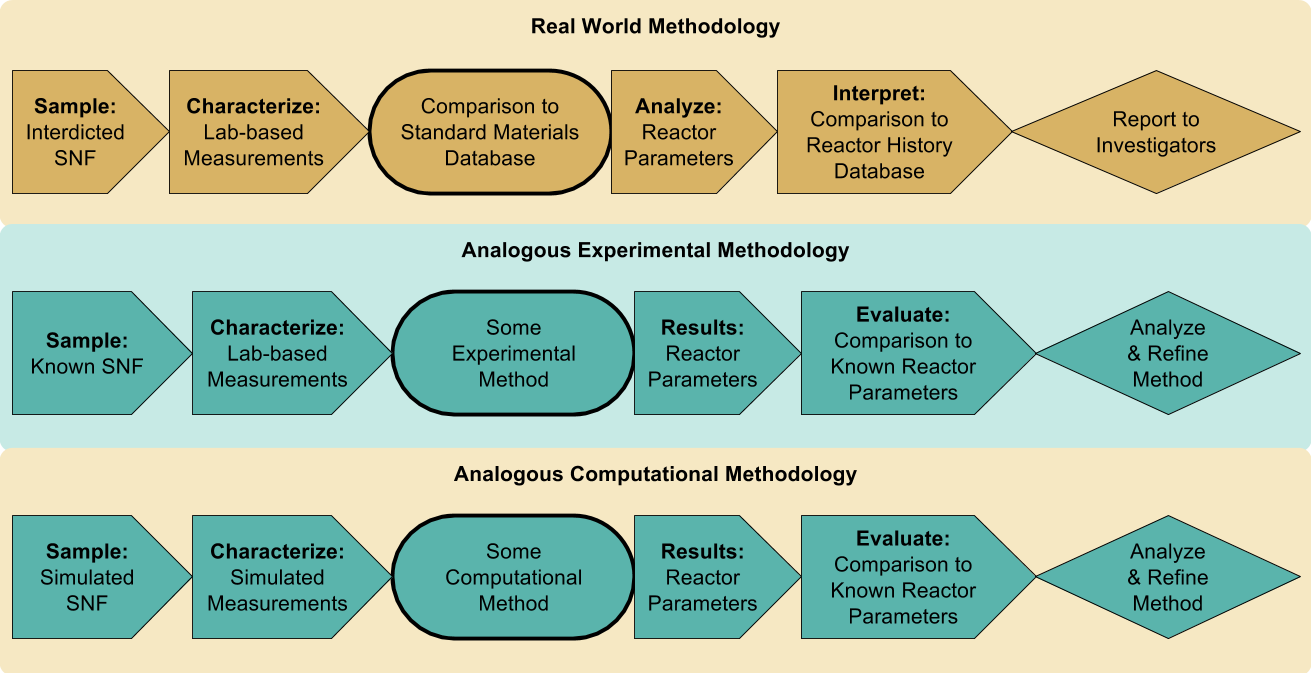
\includegraphics[width=\linewidth]{./chapters/intro/ForensicsWorkflows.png}}
  \caption{Schematic comparing nuclear forensics investigative workflow in the 
           top panel with research approaches for physical and computational 
           experiments.}
  \label{fig:nfworkflows}
\end{figure}

Next, the investigation process can be translated to an experimental workflow.
The middle and bottom panels in Figure \ref{fig:nfworkflows} are analagous
physical and computational experiments, respectively.  Both of these
experimental scenarios would have validated measurements of \gls{SNF}; the
middle panel shows this being done in the laboratory and the bottom panel shows
that these are values from a simulation. The goal of an experimental laboratory
study is to test or develop empirical relationships between forensics
signatures and the desired reactor parameters. The goal of computational
studies can be this, finding new empirical relationships, or performing
forensics workflows prior to the implementation of new reactor technologies.
For studying alternative measurement techniques or a slight difference in the
overall approach, a researcher would iterate through multiple studies using
known materials to probe sensitivities or other weaknesses in the procedure.

As mentioned, these processes have informed the experimental design of this
work, which follows the bottom panel in Figure \ref{fig:nfworkflows}. A test
sample of simulated \gls{SNF} will undergo a measurement that is computed using
techniques that mimic destructive or non-destructive measurements of nuclides
present in the sample.  Using a statistical model, the measurements are
compared to a database of \gls{SNF} entries and their reactor parameters,
finding a closest match or prediction for the test sample. Since the test
sample has previously known parameters, the error in the prediction can be
measured and the method can be tuned. 

In addition to the steps of an investigation informing the experimental
protocol, there are other considerations to take into account. In the
simulation and statistical learning paradigm, it is important to determine how
much information to what quality is needed to train an \gls{ML} model. Because
creating databases from real measurements to represent \gls{SNF} from reactor
technologies from around the world is not within the scope of this project, the
database in this study will be created from simulations via the \gls{SCALE}
\cite{scale} system using \gls{ORIGEN} \cite{origen, origenarp}. This is the
first process shown in Figure \ref{fig:intromethod}, referred to as training
data because this is what input information is called in \gls{ML}. It is
covered in Section \ref{sec:training1}.

\begin{figure}[!hbt]
  \makebox[\textwidth][c]{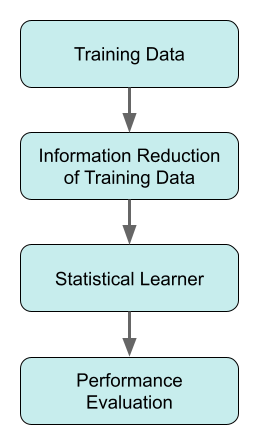
\includegraphics[width=0.3\linewidth]{./chapters/intro/methodology_intro.png}}
  \caption{Flowchart of the steps the experimental methodology for this work.}
  \label{fig:intromethod}
\end{figure}

The second process shown in Figure \ref{fig:intromethod} is information
reduction, and is detailed in Sections \ref{sec:inforeduc1} and
\ref{sec:inforeduc2}.  This refers to measurement error and/or the measurement
type that provides the nuclide information, and allows the extension of this
workflow to better mimic constraints seen in a real-world setting.  For
example, the primary example here is the reduction of information quality via
gamma ray detector, which provide less exact nuclide information than, e.g.,
mass spectrometry.  The radionuclide concentrations from the simulations can be
converted into gamma energies, which then undergo a detector response
calculation to represent real as-measured gamma spectra as closely as possible.
If an algorithm could overcome the limitations of gamma detection and still
provide useful results, this would warrant further studies and perhaps be
field-applicable.

The third step is to choose a method that performs model creation via
statistical learning.  Statistical learners have varied strengths and
weaknesses based on what is being predicted and how they implement
optimization. Introduced in Section \ref{sec:algs} and implemented in Section
\ref{sec:statmodel1} are three methods: \textit{k}-nearest neighbors, decision
trees, and \gls{MLL} calculations. The first two are implemented via a python
\gls{ML} library, scikit-learn \cite{scikit}. The \gls{MLL} method was
originally developed for similar attribution work \cite{mll_method,
mll_sensitivity, mll_validate} and was implemented in python.

After the training is complete, the results of each models' predictions must be
evaluated according to their prediction performance, denoted as the fourth
process in Figure \ref{fig:intromethod}.  The machine-learned model predicts
the parameters of a previously unseen test set.  The difference between the
model predictions and the actual simulated parameters is known as the testing
error or prediction error. This is outlined in Section \ref{sec:testerr}, and
the results are in Sections \ref{sec:eval1} and \ref{sec:eval2}.

Thus, ultimately, this research protocol is designed to answer the question
\textit{How does the ability to determine forensic-relevant spent nuclear fuel
attributes using machine-learning techniques degrade as less information is
available?}. 

\section{Goals}

The main purpose of this work is to evaluate the utility of statistical methods
as an approach to determine nuclear forensics-relevant quantities as less
information is available. \Gls{ML} algorithms (\textit{k}-nearest neighbors,
decision trees, and \gls{MLL} calculations) are used to train models to provide
these categories (reactor type) and values (burnup, enrichment, and time since
irradiation) from the available information.  The training data is simulated,
which provides an array of nuclide measurements as the features ($X$). The
prediction parameters of interest ($y$) are provided from the simulation
inputs. Information reduction on $X$ is carried out using artificially injected
random error or computationally generated gamma spectra. The prediction errors
($y_{true}$ versus $y_{pred}$) will be studied to draw conclusions about the
capability of statistical methods to inform nuclear material attribution with
less precise detection techniques.

The necessary background is covered in Chapter \ref{ch:litrev}.  First, an
introduction to the broader field of nuclear forensics is in Section
\ref{sec:nfoverview} to place this work in the context of the technical mission
areas. After that, a short discussion of the field of \gls{ML}, the algorithms
used, and model perfomance considerations are in Section \ref{sec:mlback}.
Lastly, a review of statistical methods being used in studies of forensics
analysis is covered in Section \ref{sec:stats4nf}. 

After the existing work is discussed, the first experimental procedure is
outlined in Chapter \ref{ch:exp1}: Reactor Parameter Prediction Using Nuclide
Masses.  This experiment is done as a demonstration of the methodology with the
"perfect knowledge" of nuclide masses. These measurements also undergo
information reduction by way of randomly applied uniform error. The performance
of test cases drawn from the training data is presented and discussed, as well
as the performance of real external test cases of nuclide concentration
measurements.  The methodology and implementation of the experimental
components are introduced in four subsections: the simulated training data is
in Section \ref{sec:training1}, the information reduction is in Section
\ref{sec:inforeduc1}, the details for training models are in Section
\ref{sec:statmodel1}, and the performance evaluation is in Section
\ref{sec:eval1}. Within the performance evaluation, the random error injection
results are in Section \ref{sec:randerr} and the performance using a real world
set of test cases in Section \ref{sec:sfcompo}.

Next, the second experimental procedure is explored in Chapter \ref{ch:exp2}:
Reactor Parameter Prediction Using Processed Gamma Spectra.  This experiment's
purpose is to probe the usefulness of field-deployable detectors for giving
rapid information about presumed \gls{SNF}. The information reduction is
achieved by using computational gamma spectra of various detectors with
decreasing detector energy resolution.  The performance of the prediction of
reactor parameters is measured by using test cases drawn from the training set,
where there is a training set for each detector in this study.  The methodology
follows the same workflow as the first experiment, but updates to the
components will be covered: the new training set features are in Section
\ref{sec:training2}, the information reduction from full nuclide knowledge to
processed gamma spectra is in Section \ref{sec:inforeduc2}, the changes to the
training models are in Section \ref{sec:statmodel2}, and the performance
evaluation is in Section \ref{sec:eval2}.

Lastly, the concluding remarks are discussed in Chapter \ref{ch:concl}. The
main conclusions drawn from the results in Sections \ref{sec:eval1} and
\ref{sec:eval2} are covered in Section \ref{sec:concl}. There are also many
avenues that this work does not explore and several ways to extend this work;
these are outlined in Section \ref{sec:future}.
